\chapter{基于贝叶斯的无穷远参考下脑电电势的统一估计量:正则化的参考电极标准化技术}

\section{引言}
90年来,人类脑电图对于研究认知和临床神经科学来说已经成为不可或缺的工具。超高的时间分辨率、成本较低和无创性使其成为研究大脑的有力转化工具之一。然而,两个主要缺陷:容积传导效应造成的空间混叠模糊和总是基于一种参考点\cite{teplan2002fundamentals}的电势测量的固有不确定性,减少了其探究定位脑活动的能力。空间模糊正在被先进的溯源成像技术所解决,不是本章节的重点。我们重点研究令人烦恼但不完全解决的“脑电参考电极问题上”。
为了精确定义这一问题,我们注意到这是由于脑电记录的固有本质是两个位点上的电势差。如图一所示
\begin{figure}
	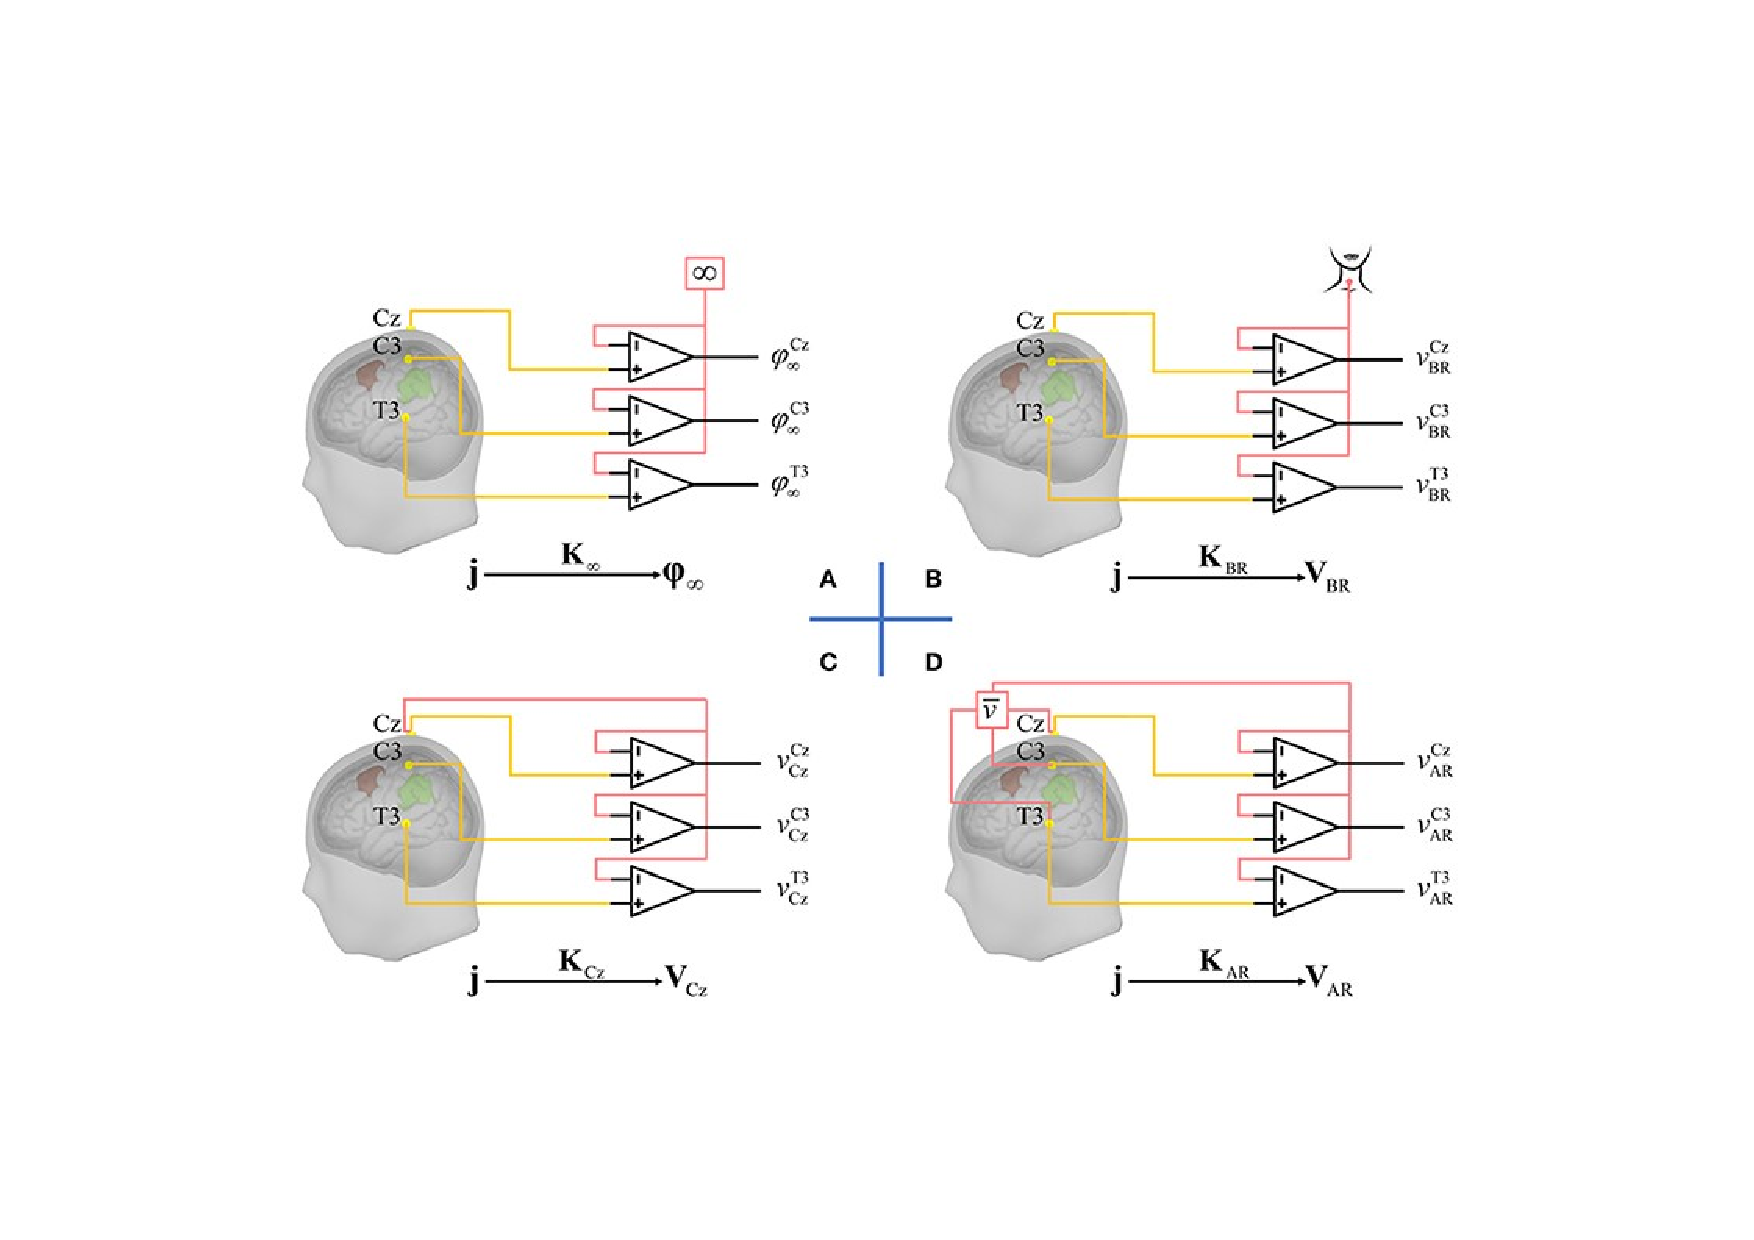
\includegraphics[width=0.8\textwidth,natwidth=610,natheight=642]{pic/3.1.pdf}
\end{figure}


\section{结果}

\section{本章小结}